\documentclass[a4papper,11pt]{article}
\usepackage[spanish]{babel}
\usepackage[utf8]{inputenc}

\usepackage{biblatex}
\addbibresource{biblio.bib}
\printbibliography


\usepackage{graphicx}
\usepackage{apacite}
\graphicspath{ {fig/} }
\usepackage{subfig}
\usepackage{siunitx}
\let\DeclareUSUnit\DeclareSIUnit
\let\US\SI
\DeclareUSUnit\inch{in}
%\usepackage[document]{ragged2e}
\title{Anteproyecto}
\author{Felipe Kiefer}
\begin{document}
  \begin{titlepage}
    \raggedright
    {
\includegraphics[width=0.3\textwidth]{ubo}\par}
    \centering
    {\bfseries\LARGE UNIVERSIDAD BERNARDO O’HIGGINS \par}
    \vspace{1cm}
    {\scshape\Large FACULTAD DE INGENIER\'IA \par}
    \vspace{1cm}
    {\scshape\Large ESCUELA DE INGENIER\'IA CIVIL INDUSTRIAL \par}
    \vspace{1cm}
    {\scshape\Large Propuesta de mejora de proceso de gestión de inventario, mediante la implementación de WMS para el caso de área de almacén del taller de servicio mecánico integral y electricidad automotriz DUARCON \par}
    \vspace{1cm}
    {\itshape\Large ANTEPROYECTO PARA SEMINARIO DE TITULO PARA LA OBTENCIÓN DEL TITULO INGENIERO CIVIL INDUSTRIAL \par}
    \vfill
    {\Large Autor: \par}
    {\Large Felipe Kiefer \par}
    \vfill
    {\Large \today \par}
  \end{titlepage}
\tableofcontents
\newpage
\listoffigures
\newpage
%1.1. Nombre del seminario:
%1.2. Fundamentos:
%1.3. Objetivo general:
%1.4. Objetivos específicos:
%1.5. Metodología:
%1.5.1. Alcances:
%1.6. Estructura:
%1.7. Carta Gantt:

\def \name {Felipe Kiefer}
\def \mlm {mercado automotor de livianos y medianos}

  \section{Nombre del seminario}
    Propuesta de mejora \cite{heizer} en \autocite{heizer} la eficiencia del uso de la \textbf{capacidad del almacén} en el proceso de gestión y control de inventario, mediante la implementación de Warehouse Management System, para el de área de almacén del taller de servicio mecánico integral y electricidad automotriz DUARCON.

  \section{Fundamentos}
    \subsection{Antecedentes, situación actual mercado automotor} 
      El \mlm a experimentado una volatilidad en sus ventas desde octubre de 2019, debido al escenario  social ocurrido en Chile, tuvo una variación negativa, se comercializaron 28.038 unidades, lo que originó una disminución en las ventas de vehículos nuevos de 24,5\% en comparación al mismo mes del año pasado.(ANAC octubre 2019)
      Este se acrecentó durante la crisis pandemia del COVID-19, Durante el mes de mayo se comercializaron 8.681 unidades de vehículos livianos y medianos nuevos, registrando una caída de 72,2\% en comparación con el mismo mes de 2019, "Estos resultados se explican, principalmente, por el deterioro de las condiciones económicas a nivel internacional que han afectado a distintos mercados, no solo el automotriz, las cuales se han visto acrecentadas por las circunstancias políticas y económicas a nivel local(ANAC Febrero 2020 pag3).
        \begin{figure}[h]
        \centering
        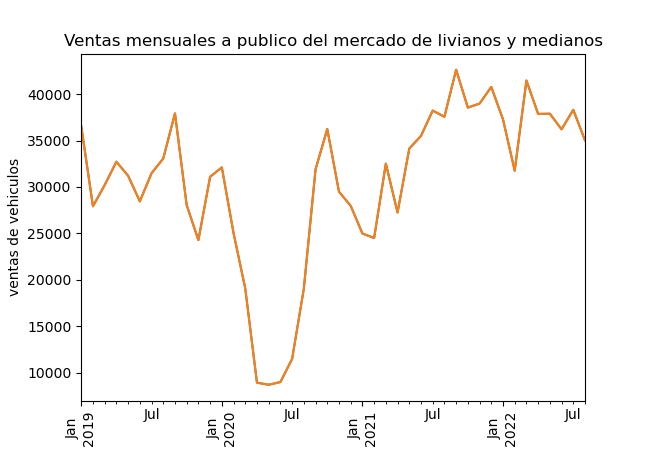
\includegraphics[width=\textwidth]{anac.png}
        \caption{Ventas mensuales a publico del mercado de livianos y medianos}
        \label{fig:anac}
        \end{figure}
      Desde el segundo semestre del 2020 \mlm crecen las ventas, diario el mercurio informa, el parque de autos se acelera y rozará los 5,5 millones de unidades este año. Esto en un contexto de mayor liquidez por los retiros del 10\% de las AFP y también del uso de vehículos para actividades laborales como las de reparto y servicios de movilización privada.
      Otra de las razones de este comportamiento, indica La Ministra de Transportes, Gloria Hutt; "El uso del auto es una reacción de las personas para sentirse más seguras. Tratan de evitar viajar en modos compartidos, pero la evidencia muestra que el transporte no ha sido un foco de contagios".
      En Marzo de 2023 continuó con la tendencia a la baja, cerrando con -9,4\% y 37.560 unidades comercializadas de vehículos livianos y medianos, esta caída fue menor a la experimentada en los meses anteriores. Este resultado está alineado con las expectativas que existen hoy en torno al desempeño económico del país con una desaceleración(ANAC Marzo 2023 pag2).
     Con respecto a lo anterior indicado podemos afirmar que el \mlm no es ajeno es a factores económicos, social ya sean nacional o internacional. nacionales e internacional. En consecuencia ante la volatilidad  de \mlm, se puede inferir que tiene un impacto en la demanda en servicios necesarios para \mlm, lo cual es un llamado para los a revisar y buscar falencia en el servicio de mantenimiento y reparación automotriz,, para transformarlas en oportunidad para enfrentar de mejor manera el comportamiento del \mlm.
 
  \subsection{Formulación de problema}
    En reparo a lo anterior, el área de bodega del taller presenta falencias debido a que no existe un sistema formal de gestión y control de inventario (WMS). Para entender algunos problemas del inventario, entendamos que es. [@Guerrero2017praxis] define inventario, como un conjunto de recursos que se mantienen ociosos hasta el instante mismo en que se necesiten [...]. Ademas agrega que [...] la sola permanencia de este inventario está generando un sin número de costos asociados. Las razones para mantener se relacionan con el servicio al cliente o para costear economías indirectamente derivadas de ello (Ronald Balong pag 328). Dependiendo del tipo de inventario que se almacena se puede justificar su existencia, o de lo contrario se estaría incurriendo en un costo innecesario y que debido a la falta de sistema de WMS no es posible alertar y también cuantificar.
    Para conocer el estado del stock en Duarcon, se realizo un inventario en junio de 2021, para una mejor apreciación a continuación se presenta un resumen de las existencias de la bodega, agrupando por tipo de producto, y de estos cuanto productos del mismo código existen.
      \begin{figure}[h]
      \centering
      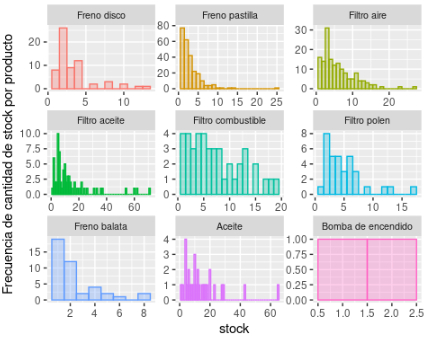
\includegraphics[width=\textwidth]{inventario.png}
      \caption{Ventas mensuales a publico del mercado de livianos y medianos}
      \label{inventario}
      \end{figure}
    
    Antes de analizar la figura \ref{inventario} se debe tener presente en general que dependiendo del tipo producto, este puede ser utilizado para distintos tipos de modelos de vehículos como es el caso de los Aceites. La figura \ref{inventario} se puede observar que algunos tipos de productos tienen un alto stock de pocos códigos de productos tale como:
    \begin{itemize}
      \item filtro de aire que se aprecia una cantidad mayor a 25 unidades
      \item filtro de aceite mayor a 75 unidades
      \item Pastilla de freno que cuenta con 25 unidades para un código, teniendo en cuenta que este producto es mas especifico para cada tipo de modelo.
    \end{itemize}

    El nivel de stock en almacén es alto, esto se refleja en la necesidad del taller de aumentar el área de almacén, por lo que en mayo de 2020 se construye un segundo almacén, por lo que el espacio utilizado para bodega que consistía de un área inicial de 418 ft^2 , se adicionan 243 ft^2, lo que da un total de 661 $ft^2$ de plaza para almacén, la figura \ref{layout} en la pagina \pageref{layout}  muestra la distribución del taller con sus respectivas medidas. 
      \begin{figure}[h]
      \centering
      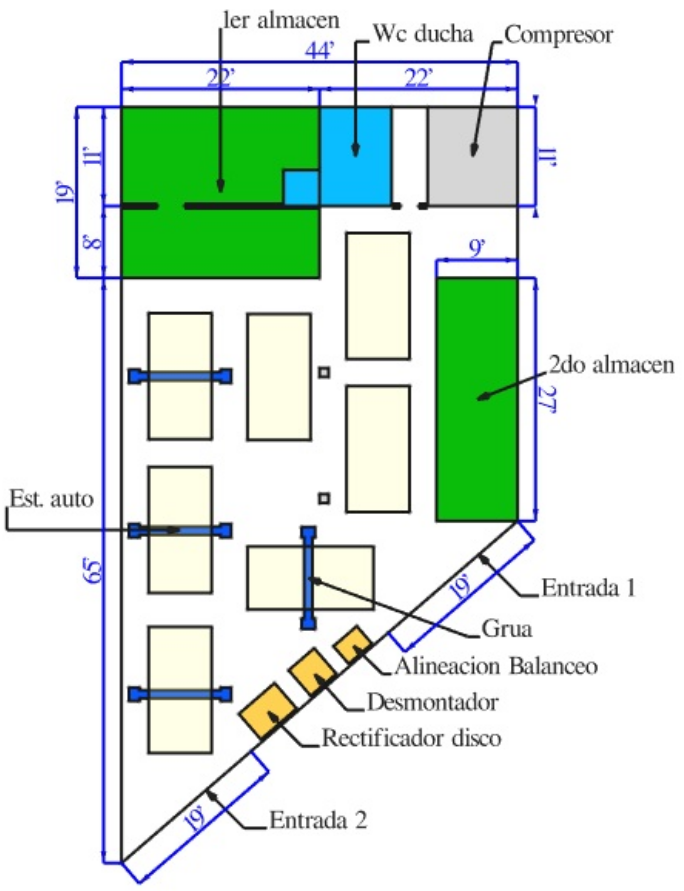
\includegraphics[width=\textwidth]{plan.png}
      \caption{Layout, Taller Duarcon}
      \label{layout}
      \end{figure}

    El estado de la bodega, representada en la figura \ref{almacen1_front}  \ref{almacen1_back} en la pagina \pageref{almacen1_front},  muestra un mantenimiento que puede ser mejorado debido a que se puede observar:

      \begin{itemize}
        \item Espacio reducido y obstruido para desplazamiento.
        \item Almacenamiento fuera de estándar
        \item Acumulación de polvo y dificultad para limpieza
        \item Dificultad para separar y clasificar espacio.
      \end{itemize}

    Estos puntos son considerados como \textbf{costo de mantenimiento} que es uno de los 4 tipos de costos que según [@Guerrero2017praxis] clasifica en:

      \begin{enumerate}
        \item mantenimiento
        \item penalización, 
        \item costo por ordenar o fijo
        \item costo variables
      \end{enumerate}
    
    Para hacer visible el costo de una mala administración de inventario clasificaremos los costos en 4 tipo, estos son: mantenimiento, penalización,costo por ordenar o fijo, costo variable según [@Guerrero2017praxis], en la practica estos están asociados unos a otros por lo cual incurrir en un costo notoriamente adicionara otro tipo de costo (como el costo de penalización con el de orden que aparece mas adelante).

      \begin{figure}
       \centering
        \subfloat[Rack A]{
         \label{14}
          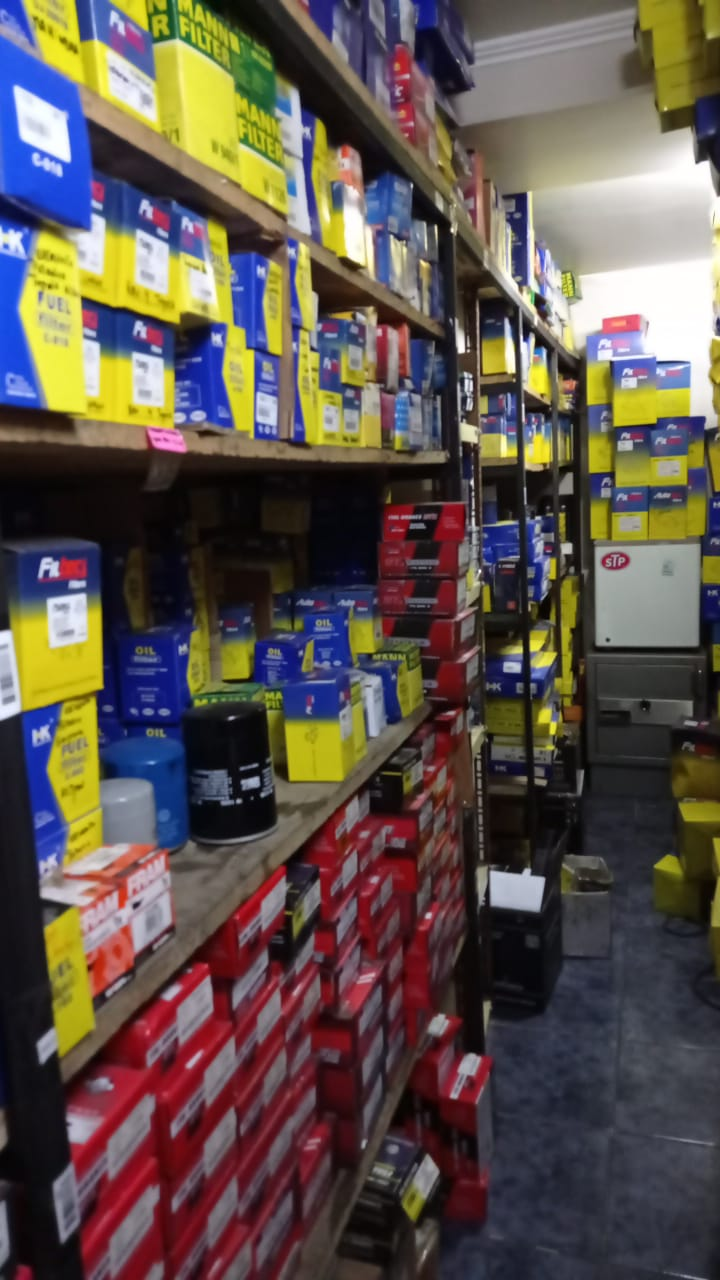
\includegraphics[width=0.3\textwidth]{14.jpg}}
        \subfloat[Rack B]{
         \label{13}
          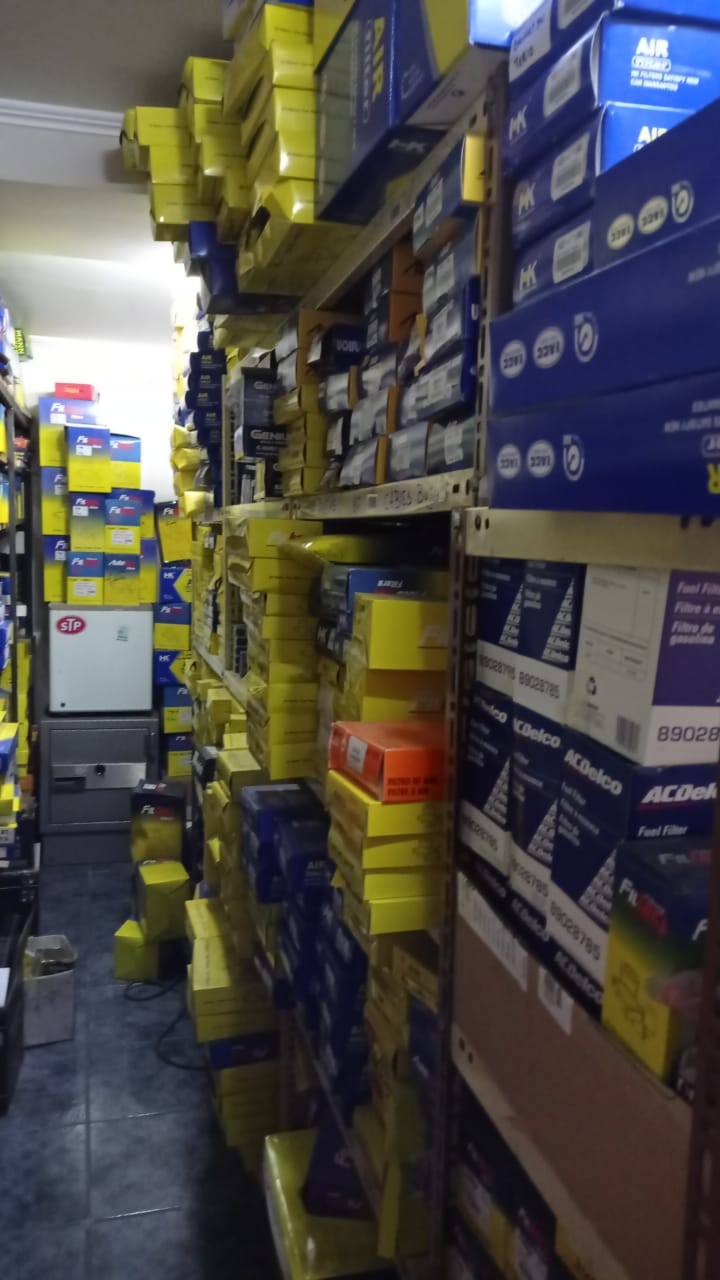
\includegraphics[width=0.3\textwidth]{15.jpg}}
        \subfloat[Rack C]{
         \label{15}
          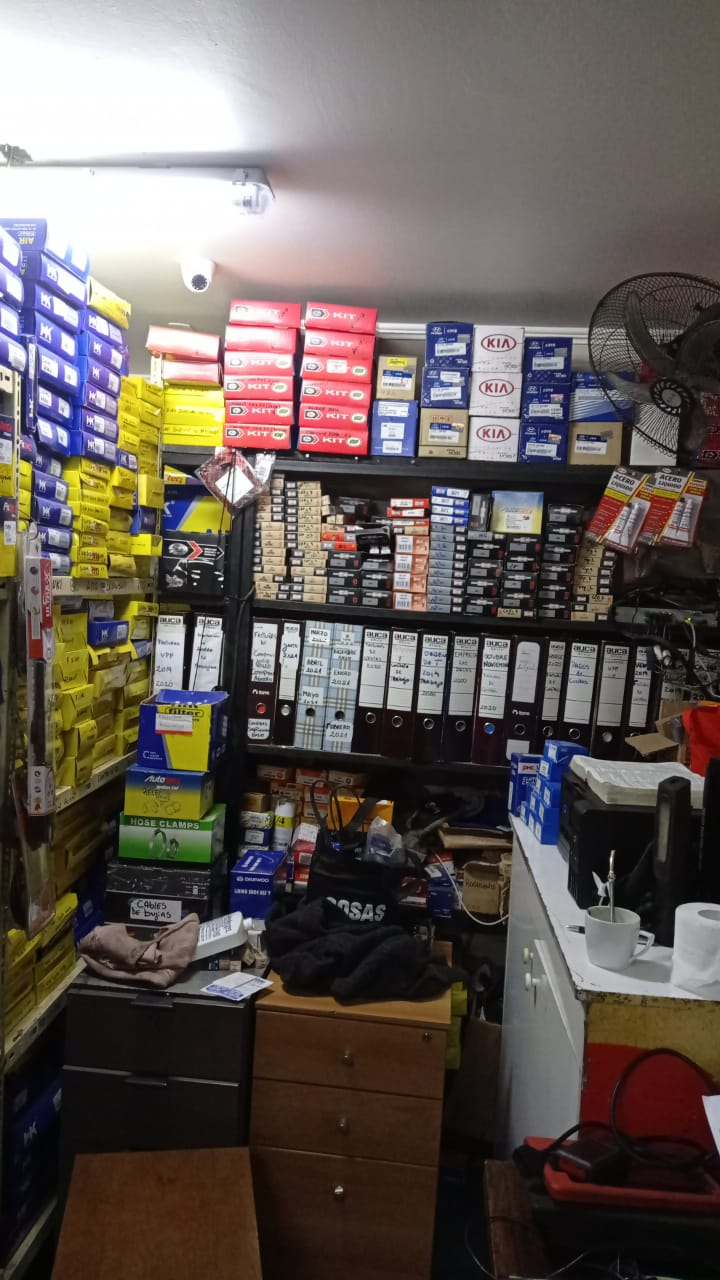
\includegraphics[width=0.3\textwidth]{13.jpg}}
       \caption{Fotografía, pasillo administración, filtros y pastillas}
       \label{almacen1_back}
      \end{figure}

      \begin{figure}
       \centering
        \subfloat[Rack D]{
         \label{18}
          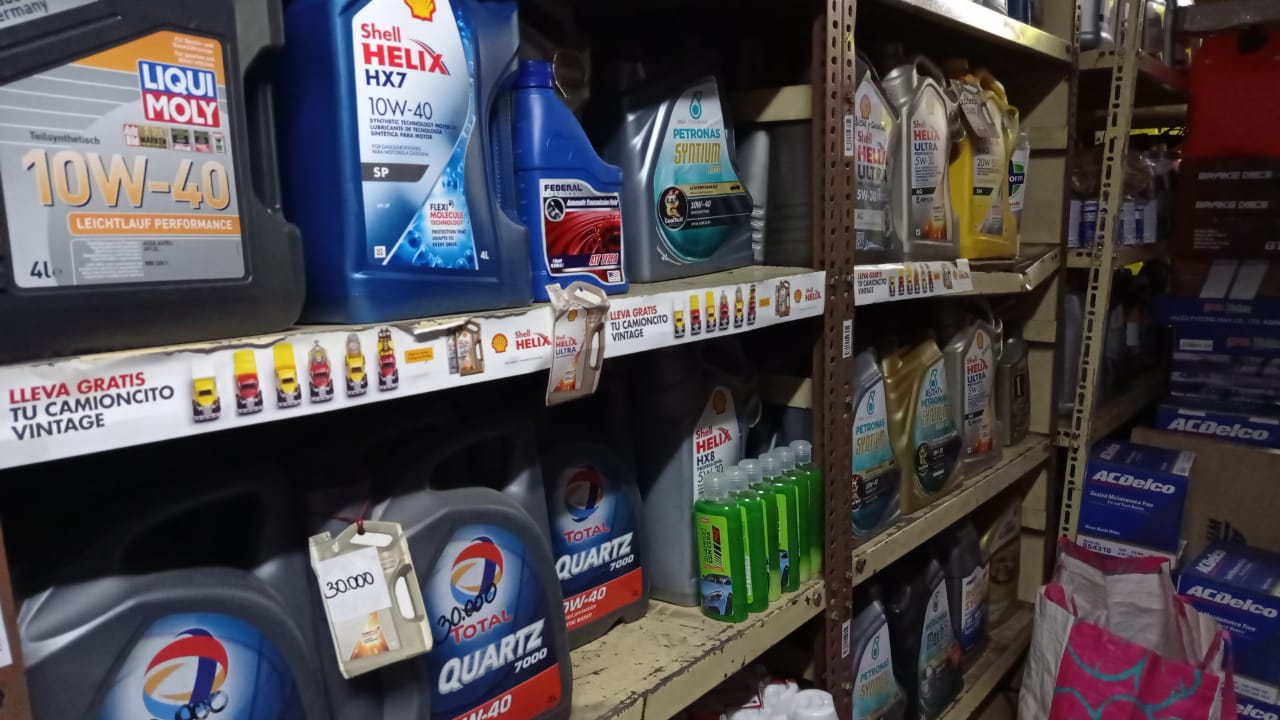
\includegraphics[width=0.3\textwidth]{18.jpg}}
        \subfloat[Rack D]{
         \label{17}
          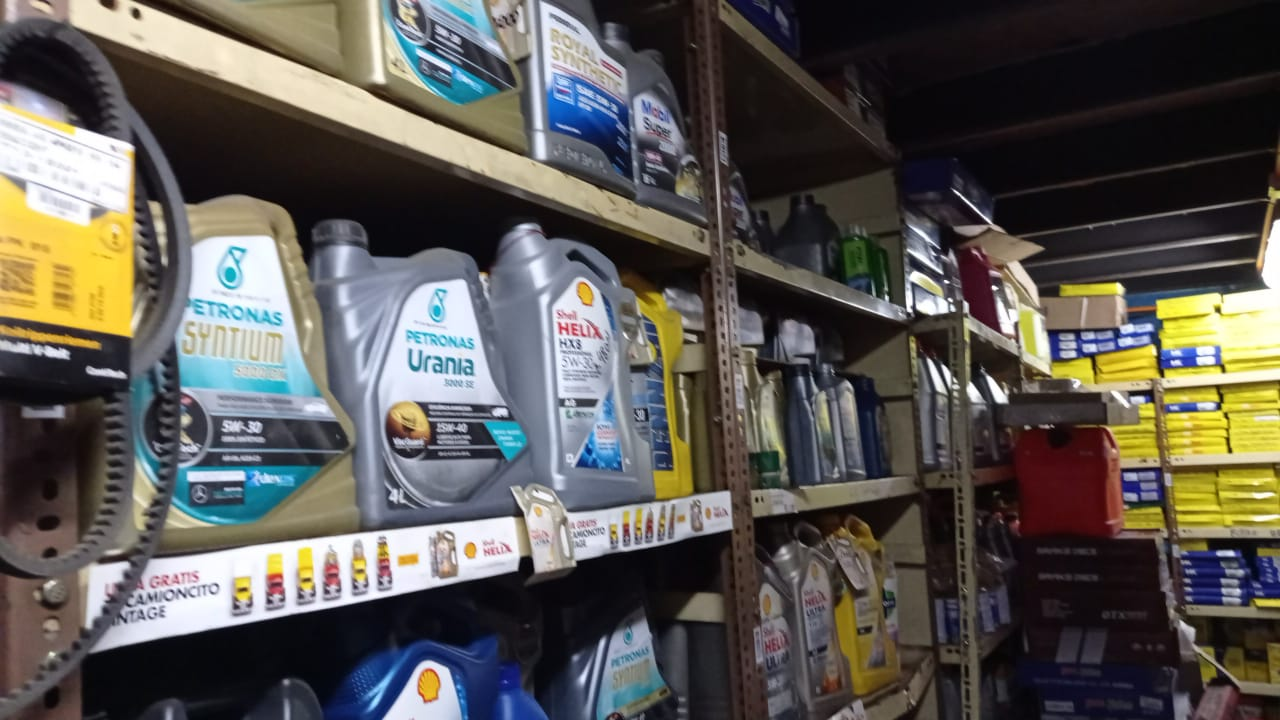
\includegraphics[width=0.3\textwidth]{17.jpg}}
        \subfloat[Rack E]{
         \label{19}
          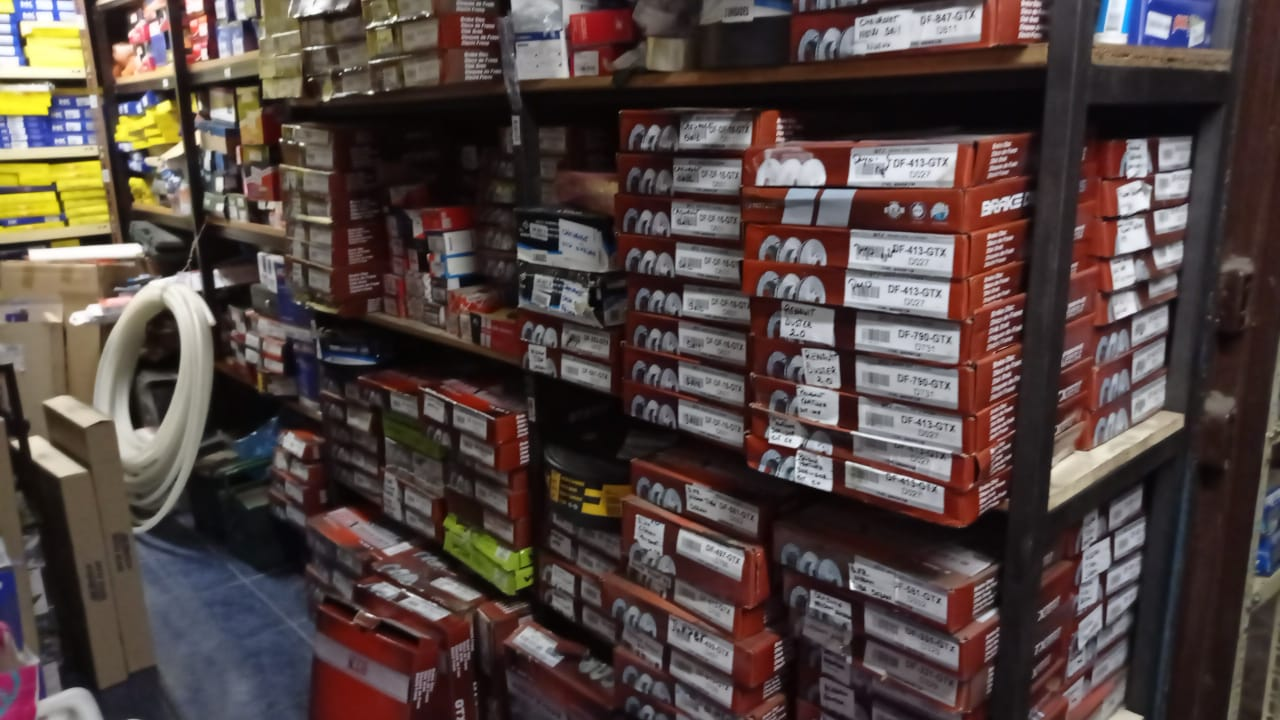
\includegraphics[width=0.3\textwidth]{19.jpg}}
       \caption{Fotografía, pasillo aceites, discos de freno}
       \label{almacen1_front}
      \end{figure}
    
    Diagrama de flujo [@Guerrero2017praxis], la importancia en el servicio
    
      \begin{figure}[!ht]
        \centering
        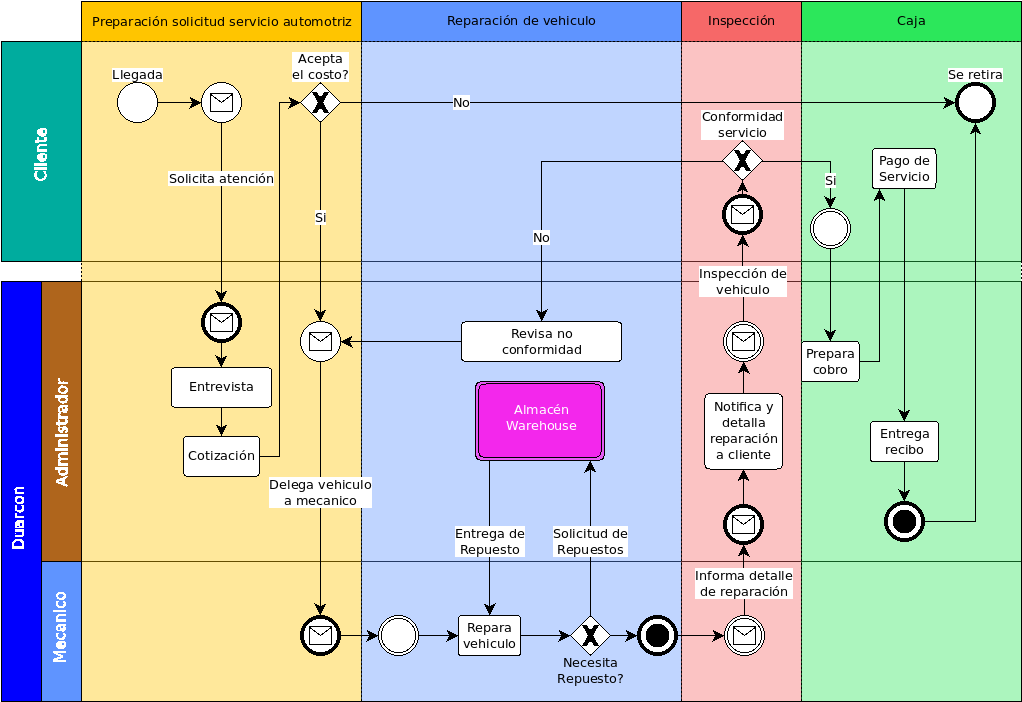
\includegraphics[width=\textwidth]{df_grl.png}
        \caption{Diagrama de flujo, servicio de reparación}
        \label{Dfl_serv}
        \end{figure}

        \begin{figure}[!ht]
        \centering
        \vspace{-20pt}
        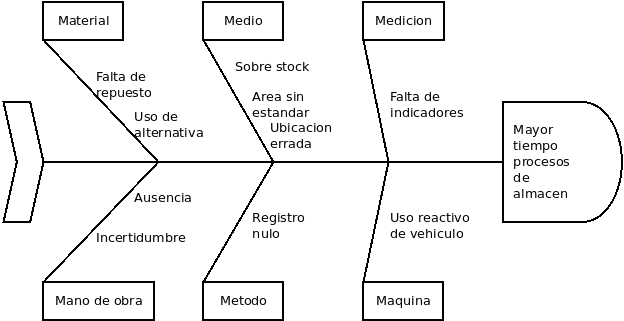
\includegraphics[width=\textwidth]{ishikawa.png}
        \vspace{-20pt}
        \caption{Diagrama de flujo, servicio de reparación}
        \label{ishikawa}
      \end{figure}


      \begin{figure}[!ht]
      \centering
      \vspace{-20pt}
      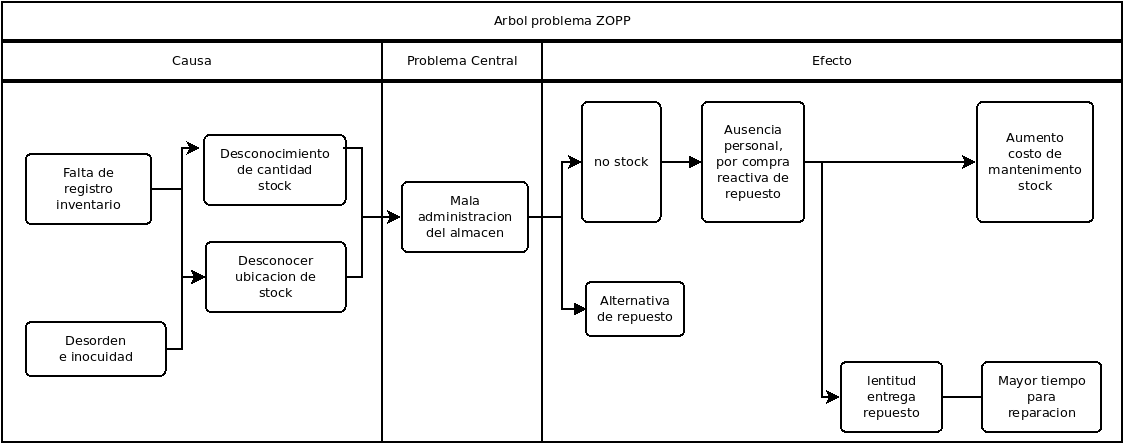
\includegraphics[width=\textwidth]{Arbol_problema_ZOPP.png}
      \vspace{-20pt}
      \caption{Diagrama de flujo, servicio de reparación}
      \label{ZOPP}
      \end{figure}

    \subsection{justificación}

    \subsubsection{porque es importante este proyecto}
      Para entender la importancia del inventario, y por que de enfocarse en ello, se señala que “el inventario es uno de los activos más costosos de muchas compañías, llega a representar hasta un 50\% del capital total invertido.[…] Por un lado, una empresa puede reducir sus costos al disminuir el inventario” (Heizer & Render, 2009, p. 484), ademas “la sola permanencia de este inventario está generando un sin número de costos asociados” (Salas, 2009, p. XVI).

    \subsubsection{cual es la problemática que intenta solucionar}
      Obtenidos los datos, se puede señalar que la problemática es de tipo metodológico (que implican un método o proceso estricto para ser solucionados), e involucra al proceso completo desde la entrada hasta la salida de stock, evidenciando la falta de control del inventario.
      “Las buenas políticas de inventarios pierden sentido si la administración no sabe qué hay disponible en su inventario” (Heizer & Render, 2009, p. 486). En consecuencia este sera la problemática a solucionar. Para la presente proyecto el objetivo es mejorar la gestión de inventario actual de Duarcon con respecto a la rapidez de y solides de la información, para ello se propone implementar una herramienta tecnológica en especifico un software, capas de registrar, controlar y entregar métodos, técnicas que otorguen al administrador capacidad de tomar decisiones concretas acerca de pedidos.

    \subsubsection{por que este proyecto y no otro}
      La realización de este proyecto es importante debido a que “Sólo cuando la organización puede determinar con exactitud qué está disponible es capaz de tomar decisiones concretas acerca de pedidos, programación y embarque”, “La exactitud de los registros permite a las organizaciones enfocarse en aquellos artículos que son más necesarios, en vez de tener la seguridad de que “algo de todo” está en inventario" (Heizer & Render, 2009, p. 486). Por lo que se puede inferir que de haber existido un sistema gestión de inventario, correcto con exactitud en los registros, habría desechado el \textbf{costo de oportunidad} de realizar de la ampliación de almacén por utilizar ese espacio en otra estación de servicio.
      El problema o efecto es el tiempo que demora la entrega de repuesto, esto debido a causas y sub causas explicado en las 6 m' (Kaoru Ishikawa), se puede observar que la causa con mas sub causas de medio, debido a que son mas visibles los problemas de este aspecto, por tanto es de esperar que también se intervenga la bodega por necesidades básicas de seguridad.
      Para abordar el problema del funcionamiento de la bodega, como objetivo se establecerá reducir el tiempo en la entrega de repuestos, ademas de proporcionar herramientas que permitan un correcto control y gestión de inventario de forma segura para el administrador, procurando no afectar el servicio de mantenimiento automotriz.

  \section{Objetivo general}
    Mejorar el tiempo de respuesta del área de almacén, implementando al proceso un software de gestión y control logístico.

  \section{Objetivos Específicos}
    Identificar situación actual, estructurar (BPM, Business Process Management), realizar medición de tiempo de cada una de sus etapas
    Estructurar el sistema de gestión de almacén e intervenir bodega para ajustarla a los requerimientos del nuevo sistema.
    Construir el proceso en base de datos (back-end), testar funcionamiento, proceder con la interfaz de usuario (front-end).
    Medir tiempo del proceso utilizando el software y comparar con las mediciones del proceso sin la utilización del software.
    Evaluar resultados.

  \section{Metodología}
    \subsection{Tipo de estudio}
      El tipo de investigación que se aplico fue descriptivo, porque describe la problemática actual que atraviesa la bodega del taller por la falta de un sistema de inventario, ademas de exploratoria porque permite participación, para posteriormente obtener los datos suficientes.
  \subsection{Método de investigación}
    Los métodos utilizados en la presente investigación son:
    Metodología explicativa: Se realizara una técnica explicativa que consiste en buscar el por qué de los hechos mediante el establecimiento de relaciones causa-efecto.
    Metodología descriptiva: Los datos son obtenidos directamente del proceso, la información es recopilada a través de la observación mientras se realizan las actividades de manera normal, ademas se realizará una entrevista al personal, acerca de la experiencia de la mejora de proceso.
  \subsection{Fuentes y técnicas para la recolección de información}
  \subsubsection{Fuentes Primarias}
    Para la recolección de la información se usará la técnica de observación directa, la cual consiste en observar, y medir atentamente las actividades laborales que se realizan en la Bodega del Taller. Esto se realizará sin obstaculizar ni intervenir en el ambiente de trabajo para que la recolección de datos sea veraz. Después se realizará una entrevista al personal de la bodega, en donde se hará una serie de preguntas las cuales, con base a las respuestas del personal, serán tabuladas para detectar las áreas con problemas, para que sean analizadas y a su vez desarrollar una posible solución.
  \subsubsection{Fuentes Secundarias}
    Otro método para la recolección de datos, ya inventariado se revisara el comportamiento del stock, ubicación, clasificación, ademas se solicitara el acceso a datos de recepción y despacho, esto para generar información útil para el desarrollo de la presente propuesta.
  \subsection{Tratamiento de la información}
    La información resultante del proceso de investigación será procesada, analizada utilizando las distintas herramientas de  TQM (Total Quality Management; administración de la calidad total), para identificar y priorizar en las principales causas que originan el problema a tratar durante el desarrollo de la presente propuesta. A continuación, se mencionarán algunas herramientas que se utilizarán en la investigación:
  
  \subsubsection{Análisis causa y efecto}
    Para identificar problemas de calidad y puntos de inspección el diagrama de causa y efecto, también es conocido como diagrama de Ishikawa o diagrama de espina de pescado. Ilustra un diagrama de este tipo (observe que la forma es parecida al esqueleto de un pez) para un problema cotidiano de control de calidad. Cada “hueso” representa una fuente posible de error.(p205)
  \subsubsection{Diagrama de Pareto}
    Las gráficas de Pareto son un método empleado para organizar errores, problemas o defectos, con el propósito de ayudar a enfocar los esfuerzos para encontrar la solución de problemas. Tienen como base el trabajo de Vilfredo Pareto, un economista del siglo XIX. Joseph M. Juran popularizó el trabajo de Pareto cuando sugirió que el 80\% de los problemas de una empresa son resultado de sólo un 20\% de causas.(p206)

  \subsection{Diagrama de flujo}
    Los diagramas de flujo presentan gráficamente un proceso o sistema utilizando cuadros y líneas conectadas. Son sencillos, pero excelentes cuando se busca explicar un proceso o se pretende que tenga sentido [@prod, pp. 207].
  \subsubsection{Transformación digital}
    Es la aplicación de capacidades digitales a procesos, productos y activos para mejorar la eficiencia, mejorar el valor para el cliente, gestionar el riesgo y descubrir nuevas oportunidades de generación de ingresos[@Baz].
  \section{Alcance}
    Este proyecto propone mejorar el proceso de gestión de inventario de almacén, hacer visibles los problemas actuales que de la gestión del almacén y los costos que acarrea, por lo que se tendrá acceso a registros de recepción y despacho durante el periodo 2020, 2021, 2022, ademas del stock existente. Se intervendrá el espacio físico de la bodega dependiendo de los requerimientos de la mejora.
    Con respecto a los trabajadores, se pretende motivar a los colaboradores adoptar métodos que involucren la calidad en el proceso, y que posterior al desarrollo de este proyecto, incentive a mejoras en otras áreas del servicio.
  \section{Estructura}
    La estructura sería preliminarmente de la siguiente manera:
    
    Título.

    Dedicatoria.

    Agradecimientos.

    Índice de contenido.

    Índice de tablas y figuras.

    Resumen.

    Introducción.

    Objetivos.

    Objetivo general.

    Objetivos específicos.

    Marco teórico.

    Metodología.

    Resumen capitular.

    Desarrollo del trabajo.

    Conclusiones y/o recomendaciones.

    Bibliografía.

    Anexos.

  \section{Carta Gantt}

\pagebreak
\section{Nombre del(los) memorista(s)}

Nombre:     Felipe Kiefer

Rut:        17.414.046-4

Firma

\subsection{Profesor Guía}

Nombre:

Rut:

Firma

\subsection{Malla Curricular}

Malla año 2010

\pagebreak

\section{Referencias}
\printbibliography

% \bibliographystyle{apacite}
% \bibliography{biblo.bib} 
\end{document}
